% Author: Till Tantau
% Source: The PGF/TikZ manual
\documentclass{article}

\usepackage[latin1]{inputenc}
\usepackage{tikz}

% GNUPLOT required
\begin{document}
\pagestyle{empty}


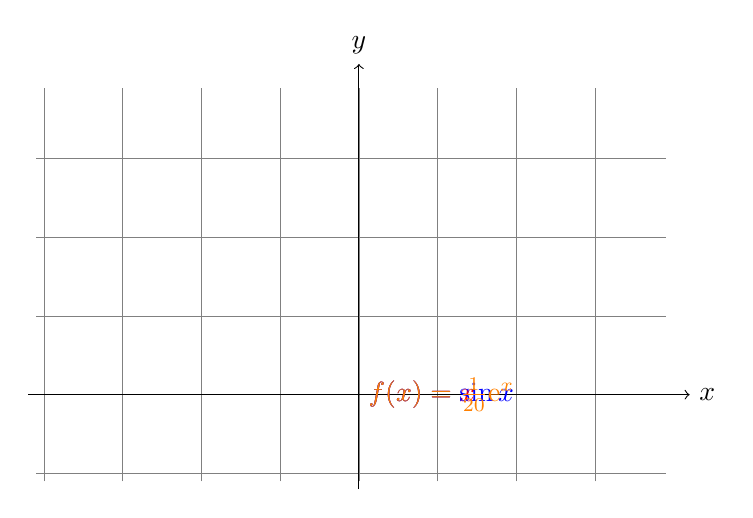
\begin{tikzpicture}[domain=-4:4]
    \draw[very thin,color=gray] (-4.1,-1.1) grid (3.9,3.9);
    \draw[->] (-4.2,0) -- (4.2,0) node[right] {$x$};
    \draw[->] (0,-1.2) -- (0,4.2) node[above] {$y$};
    \draw[color=red] plot[id=x] function{1/4.0*x**2} 
        node[right] {$f(x) =x$};
    \draw[color=blue] plot function{sin(x)} 
        node[right] {$f(x) = \sin x$};
    \draw[color=orange] plot function{0.05*exp(x)} 
        node[right] {$f(x) = \frac{1}{20} \mathrm e^x$};
\end{tikzpicture}


\end{document}
